% !TeX root = ../thuthesis-example.tex

\chapter{\MakeUppercase{The VR-IoT Research Platform}}

In this chapter, we introduce key implementation details and the structure of the VR-IoT research platform, or, as it was later named, ``NUIX-Studio.'' Firstly, we will give the requirements for the platform architecture, then we will outline the key details in its development.

\section{Platform requirements}

Our platform must provide an interface for different interaction techniques and simulation of device sensors inside Virtual reality. The device controls can be divided between touch interface interaction and other interaction methods, such as voice control, sight control, gesture control, etc. The ability to control devices at a distance impossible in real life, such as lengthening arms, dropping hands, etc., was placed in a separate category. These control methods could be used in the real world in the future by introducing new technologies such as holographic projection. 

However, in addition to handling interactions with devices, our platform must also serve as an IoT platform for connections of various IoT devices. Based on the literature review, NUIX-Studio must fulfill these minimum requirements:
\begin{enumerate}
\item Scalability. The performance of the platform should stay acceptable when the number of devices in the system increases. Otherwise, the latency of the synchronization between the devices inside the VR-IoT environment will increase to a level at which the system is unable to perform Data analysis for the research;
\item Ease of use and testing. Researchers need to be able to efficiently use the NUIX-Studio API and platform tools to create new IoT devices and test them in the VR-IoT environment.
\item Fault Tolerance. The platform should effectively handle faults coming from both real and virtual worlds to provide a satisfying user experience;
\item Simultaneous work. As in the real world, where several people can interact with an IoT system at the same time, each of the platform's running instances should be able to operate simultaneously and with the same data.
\end{enumerate}

By dividing the NUIX-Studio structure into these three layers, the platform becomes more resilient (Figure~\ref{fig:BasicPlatformStructure-figure}): 
\begin{enumerate}
    \item Real-world IoT devices HUB is a special device responsible for receiving and sending data to real-world devices that provides the data in a unified format (through the abstraction of sensors) for the middle layer. An open-source software openHAB~\cite{OpenHab} is used to support different IoT devices. The HUB runs on a server and is responsible for storing the IoT devices' data. The data is managed through a Web Interface;
    \item Integration layer is responsible for analyzing data coming from VR and the real-world, integrating real-world device data into VR (and vice-versa), performing persistence, and providing an API for using the platform in research projects. By receiving and sending unified data objects representing the IoT devices' sensor data using REST API calls, each of the NUIX-Studio App instances operates with the same data, enabling simultaneous work. The next step is to represent the IoT devices' data in Virtual reality and perform computations for research. Since the platform should run smoothly on VR headsets and provide good UX, the analysis should be performed on a powerful PC\footnote{In Chapter 4 an experiment proving this statement is provided.}. At the same time, Virtual reality headsets perform computations for interacting with objects, such as hand recognition;
    \item Visualization layer provides interaction with digital IoT devices using VR headsets, AR devices, or by simulating touch, sight, gestures, and other interactions. Developers can integrate additional interaction techniques into this layer using the NUIX-Studio Development kit, but developing these techniques is not the focus of this research. We decided to use Unity~\cite{Unity} for interaction with virtual reality devices. Firstly, Unity comes with a ready-to-use 3D engine, relieving the need to develop a new one. Secondly, Unity is multi-platform and supports VR headsets. Thirdly, developers are already familiar with Unity development, making it easier for them to integrate the platform into their solutions.
\end{enumerate}

\begin{figure}
  \centering
  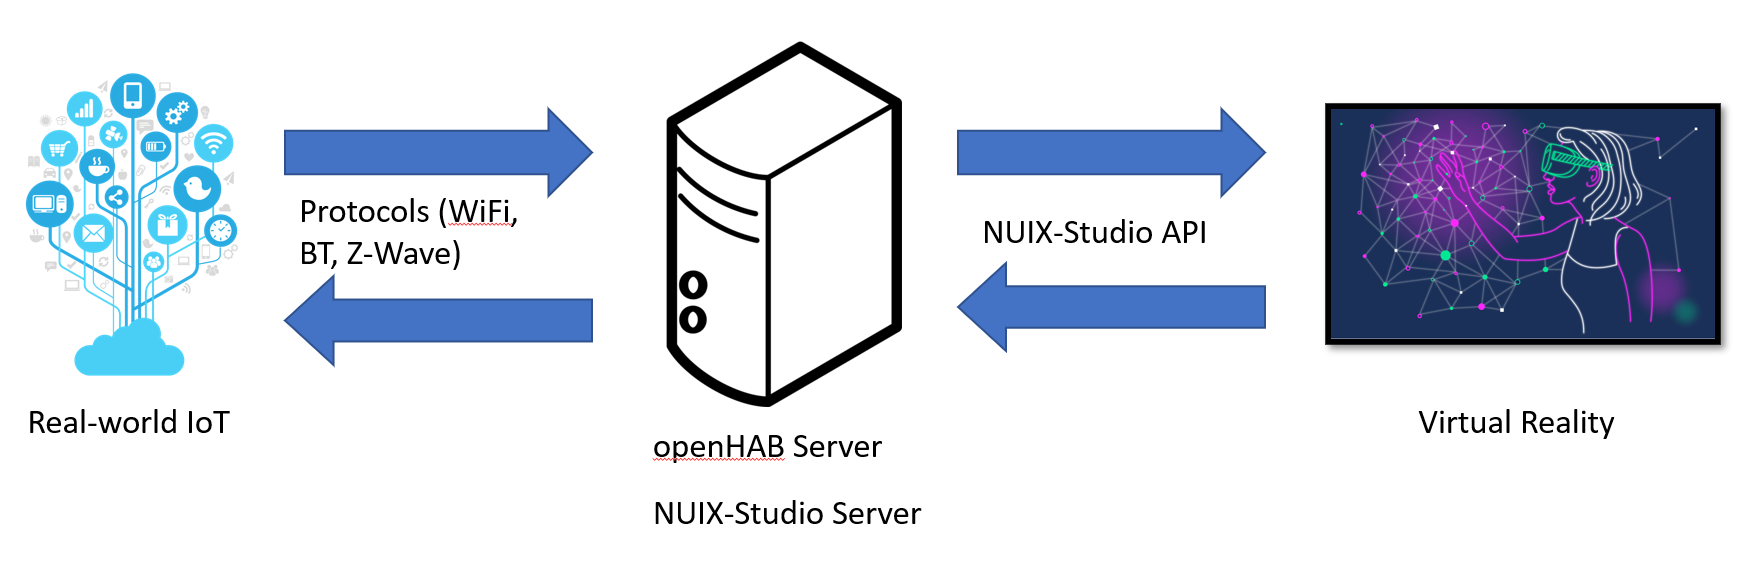
\includegraphics[width=1.0\linewidth]{figures/BasicPlatformStructure.png}
  \caption{Simplified structure of NUIX Studio. The real-world IoT devices HUB is an openHAB server, while NUIX-Studio server is an instance of the NUIX-Studio App responsible for the computations.}
  \label{fig:BasicPlatformStructure-figure}
\end{figure}

As it can be seen on the IoT-VR Platform design architecture, the Real-world IoT devices Hub should collect the data coming from IoT Services and store it in a database (Figure~\ref{fig:StructureVersion2-figure}). It should be able to synchronize the data with the integration layer, complementary linking real and virtual sensing data.

\begin{figure}
  \centering
  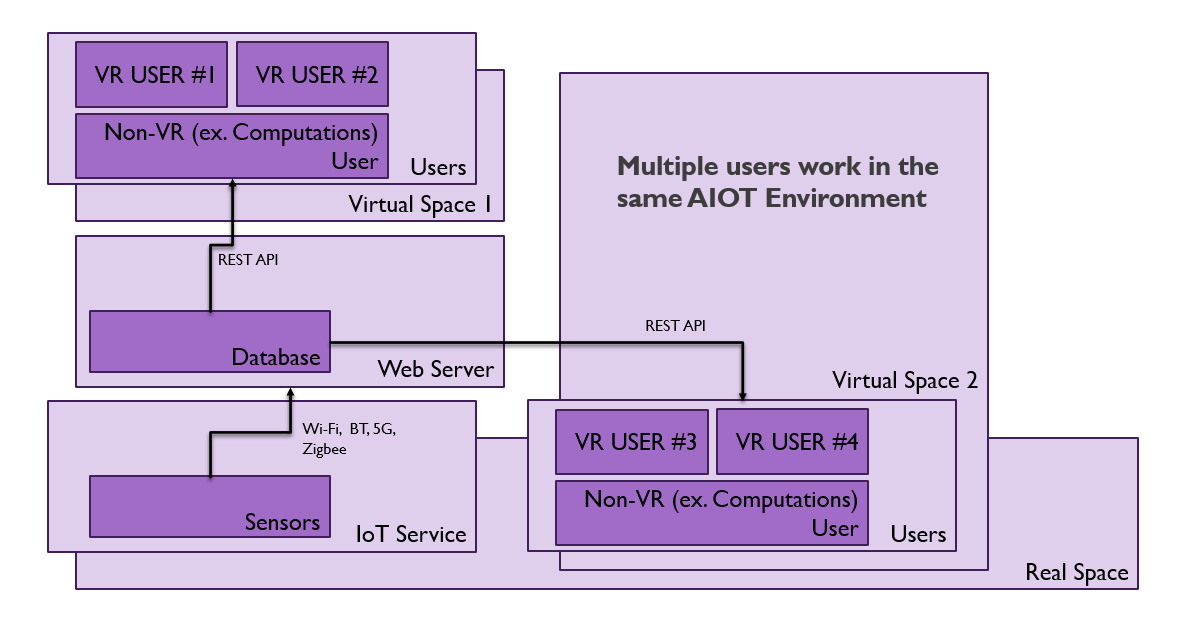
\includegraphics[width=0.9\linewidth]{figures/StructureVersion2.png}
  \caption{Design architecture of the platform for virtuality-reality synchronization and simultaneous work support.}
  \label{fig:StructureVersion2-figure}
\end{figure}

\section{Server Architecture}

\subsection{OpenHAB Server Structure}

We decided not to change the openHAB system's structure, because it already follows the SOA principles that allow implementing support for various types of devices (Figure~\ref{fig:openHABServerStructure-figure}) through unified representation of their parameters. In openHAB terminology, each IoT device is called a Thing, but a Thing can also be a service. For example, a smoke sensor or a user location are both Things. Things expose their capabilities through Channels. For example, smart vacuum cleaner channels can be suction strength, water delivery strength, remaining charge level, and cleaning status. Each channel is associated with one or more Items that are added inside the model. Items have a State, and they may receive commands. 

Before adding an IoT device to the server, the developer has to first install a software adapter. These add-ons are called Bindings, and they provide a way to link Items to physical devices. Most of the protocols for connecting to IoT devices are supported by the corresponding Bindings. For example, after a Binding for Xiaomi smart home devices is installed, the smart home devices can be automatically discovered by the server and added as Things. A Xiaomi Lamp is used in the example, for which several Channels are presented (Figure~\ref{fig:XiaomiLampChannels-figure}). Each of these channels represents one Item (Figure~\ref{fig:XiaomiLampPowerItem-figure}).

\begin{figure}
  \centering
  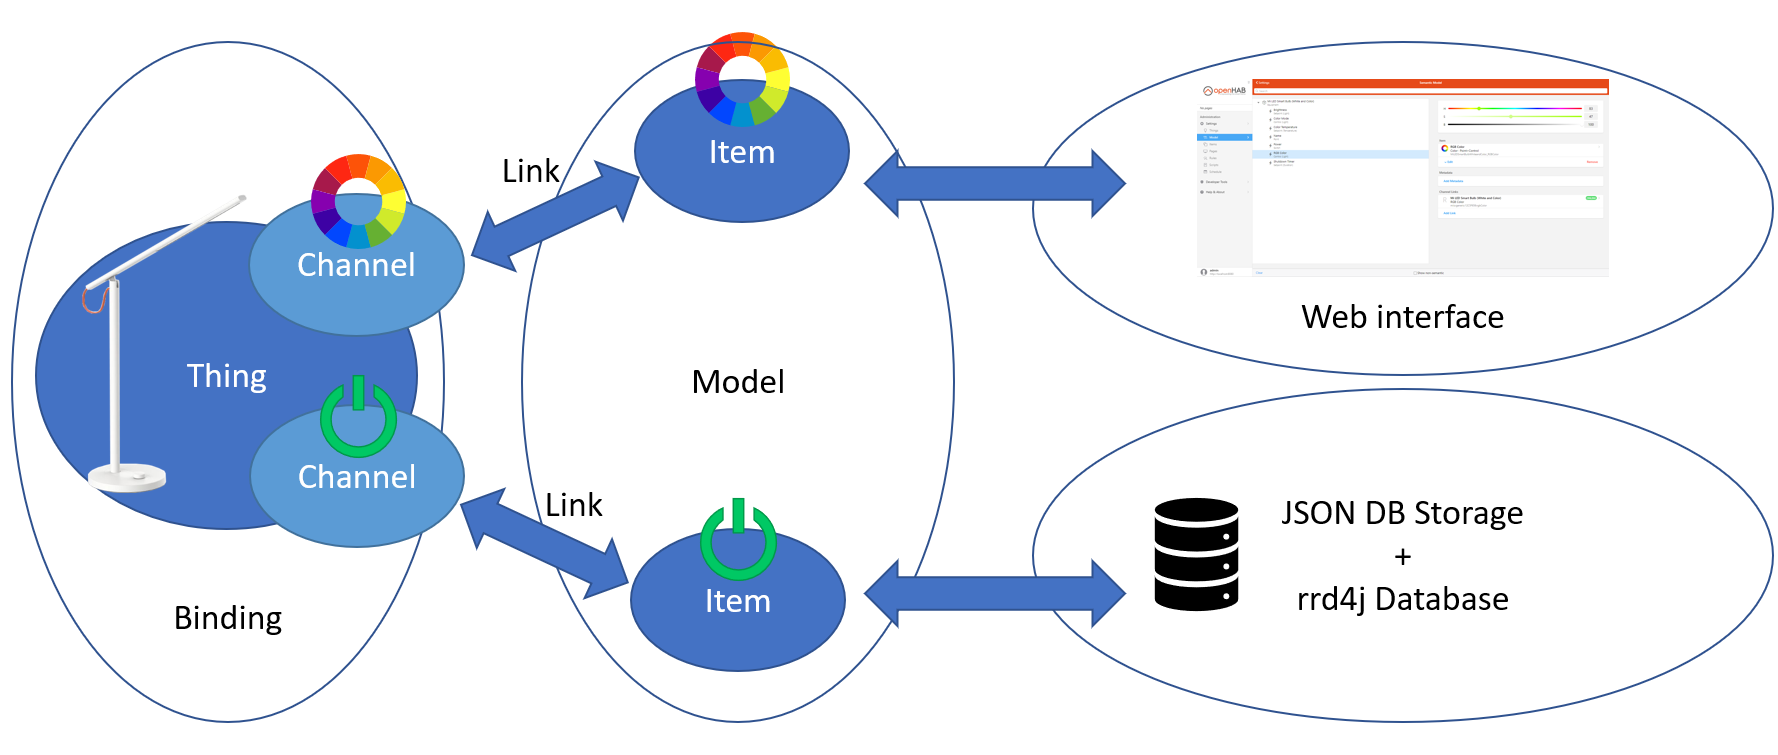
\includegraphics[width=0.9\linewidth]{figures/openHABServerStructure.png}
  \caption{Server structure}
  \label{fig:openHABServerStructure-figure}
\end{figure}

\begin{figure}
  \centering
  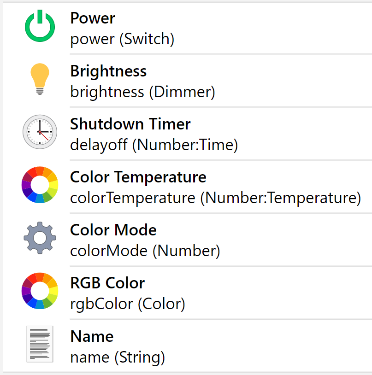
\includegraphics[width=0.6\linewidth]{figures/XiaomiLampChannels.png}
  \caption{Channels list example.}
  \label{fig:XiaomiLampChannels-figure}
\end{figure}

\begin{figure}
  \centering
  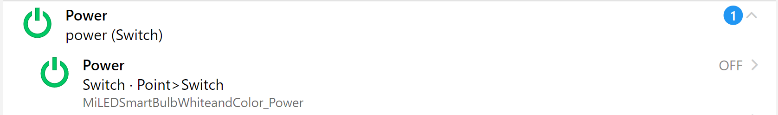
\includegraphics[width=0.9\linewidth]{figures/XiaomiLampPowerItem.png}
  \caption{An Item example. The Power Control is performed through the power channel. In terms of the introduced concepts, the Power Control is an Item named ``MiLEDSmartBulbWhiteandColorPower'' of type Switch and State ``OFF.'' As soon as the lamp is turned On, the Power Control switch in the Web Interface will also turn ON. And if the switch is changed to the ``OFF'' state in the Web Interface, the lamp will automatically turn off.}
  \label{fig:XiaomiLampPowerItem-figure}
\end{figure}

\subsection{Server Extended Structure}

Server data is synchronized with Integration layer through REST API (Figure~\ref{fig:ExtendedServerStructure-figure}), which is explained in detail in Table~\ref{tab:rest-api-table}. In the current implementation of the platform, four different REST API commands are used: GET command for receiving Items in the registry on system startup, PUT command to create a new Item on the server, POST command for updating the state of the Item, and DELETE command for removing an Item from the server.

\begin{figure}
  \centering
  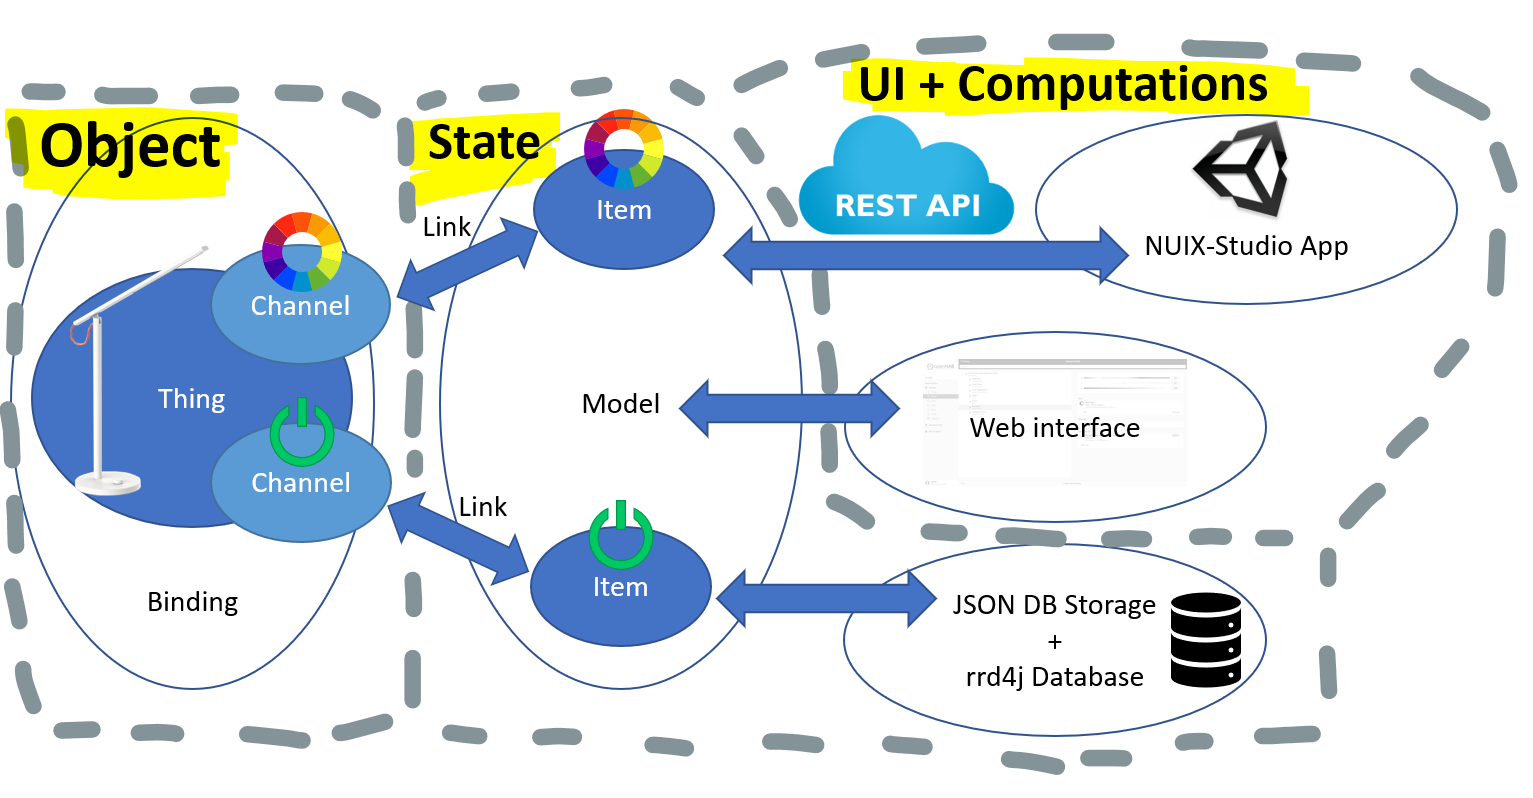
\includegraphics[width=0.9\linewidth]{figures/ExtendedServerStructure.png}
  \caption{Structure of the server showing how the NUIX-Studio App connects to it.}
  \label{fig:ExtendedServerStructure-figure}
\end{figure}

\begin{table}
  \centering
  \begin{threeparttable}[c]
    \caption{REST API commands used in NUIX-Studio}
    \label{tab:rest-api-table}
    \begin{tabular}{ll}
      \toprule
      REST API CALL    &         DESCRIPTION                 \\
      \midrule
      GET\tnote{a} & Get all available items \\
      POST\tnote{b} & Adds a new item to the registry or updates the existing item    \\
      PUT\tnote{b}        & Sends a command to the item                              \\
      DELETE\tnote{b}        & Removes an item from the registry          \\
      \bottomrule
    \end{tabular}
  \end{threeparttable}
\end{table}

States of the Items are received by getting events from the server: once the event is received, the Item state can be retrieved from the Data Transfer Object's (DTO) payload. Only updated data is transferred between Real-world devices HUB and Integration layer. 


\section{Platform architecture}

As mentioned above, there can be several NUIX-Studio App instances running at the same time. Each of them has access to the Server through REST API. The instances can be of one of the three types:

\begin{enumerate}
    \item Virtual Reality Instance. It runs on Oculus or another VR headset and has remote or local access to the server. Items received from the server are visualized. It is possible to interact with the Items in different ways by touching buttons, moving sliders, performing hand gestures, using voice commands, etc. 
    \item Computations Instance. It runs on a powerful machine and has either remote or local access to the server. Since latency is important for the VR-IoT platform's performance, it is preferable to run this instance on the same machine as the openHAB server. In this case, the REST API calls time will be less than the minimum measurement unit (compared to milliseconds for accessing remote virtual reality instances)\footnote{An experiment to prove this statement is provided in Chapter 4.}. Physics, Big Data analysis, and other performance-based computations are executed in this instance, while user interactions are limited.
    \item Input simulation instance. If the App instance runs on the device with limited support of virtual reality interaction interfaces (for example, a PC), input simulation can be used. Sometimes, it is even easier to run and test the platform on such devices: for example if using a physical keyboard is required or if there is no access to a VR headset.
\end{enumerate}

Each of the instances has access to the same data on the server, making it possible to work simultaneously in one virtual environment and divide tasks between several NUIX-Studio App instances (Figure~\ref{fig:AppInstances-figure}). One of the instances can be used for computations, while others can be used for interacting with the devices in Virtual reality.

\begin{figure}
  \centering
  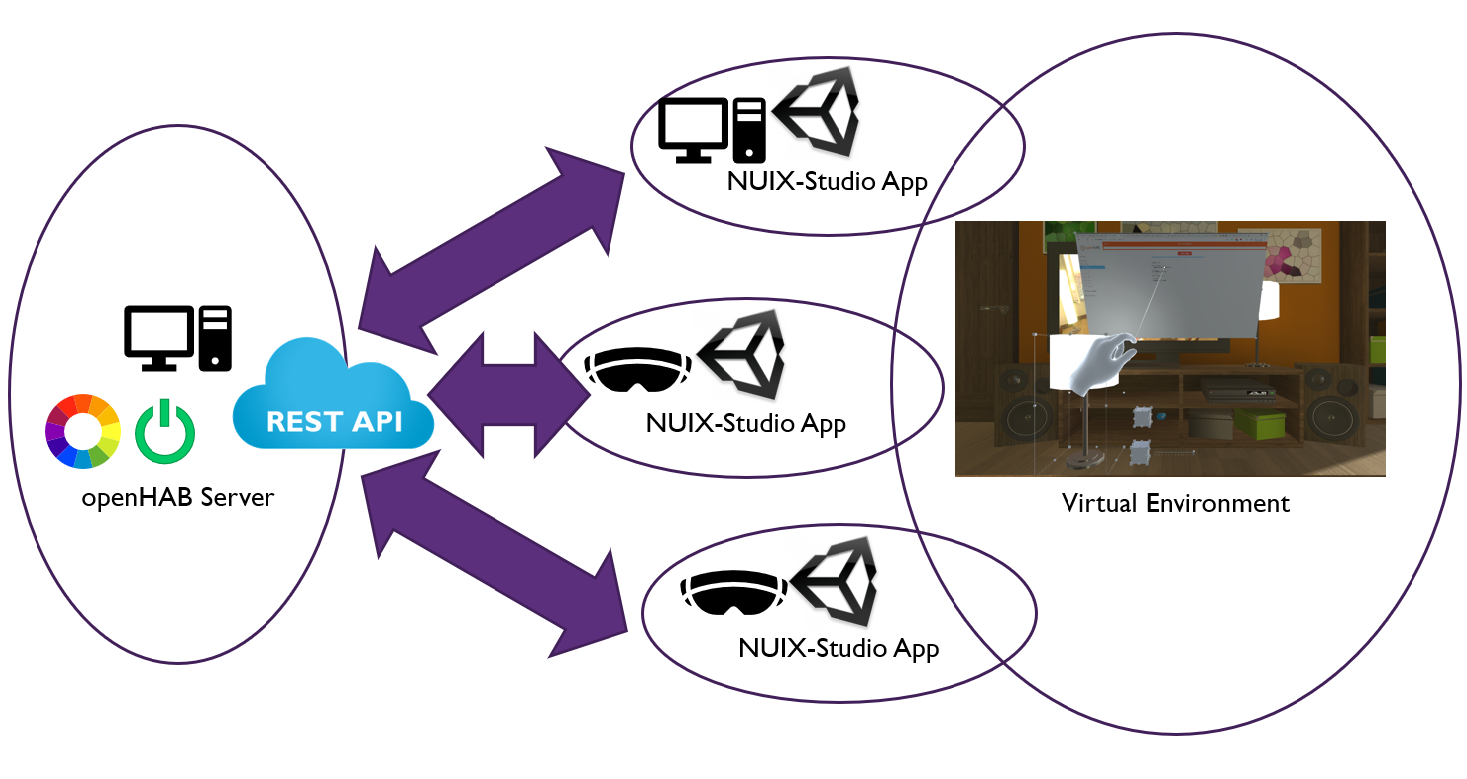
\includegraphics[width=0.9\linewidth]{figures/AppInstances.png}
  \caption{NUIX-Studio App Instances}
  \label{fig:AppInstances-figure}
\end{figure}

\subsection{NUIX-Studio App Architecture}

After the NUIX-Studio App requests access to the system to get the list of items from the registry, a list of Item Data Transfer Objects is received by the App and then added into the Semantic Model (Figure~\ref{fig:AppArchitecture-figure}). After the Item state is updated or an Item is added or removed, an event is sent to the EventController instance, and then, based on the event payload, the Item list is updated.  By keeping the Item data on the device equal to the Item data on the server, the Semantic model in the NUIX-Studio App remains equivalent to the Semantic model presented on the server. 

\begin{figure}
  \centering
  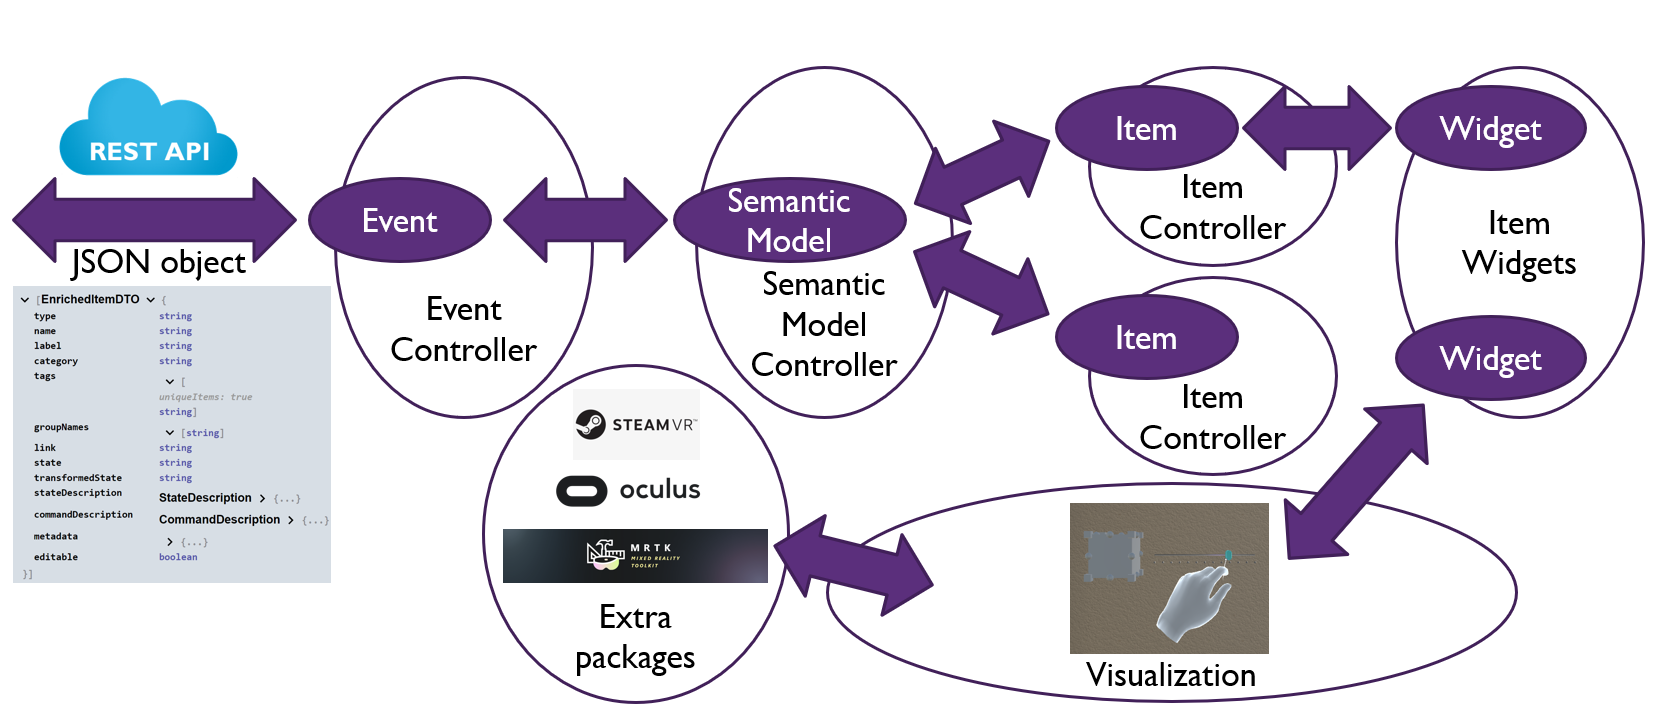
\includegraphics[width=0.9\linewidth]{figures/AppArchitecture.png}
  \caption{NUIX-Studio App Architecture}
  \label{fig:AppArchitecture-figure}
\end{figure}

But if the states of the Items are only stored in the App, users will not be allowed to interact with the IoT devices. In other words, the NUIX-Studio App has to provide an interface to interact with the Items. Since different types of Items require different interaction techniques, a Widget object is created for each item type. Widget in NUIX-Studio App is a Unity Virtual object, which can visualize the Item state and update it. For example, it can be an interactable pinch slider for a dimmer Item or a virtual screen for an Image item. By integrating Extra frameworks, the NUIX-Studio platform can provide a wider variety of Widgets and a higher number of supported devices. For example, Oculus Integration support provides an API for hand recognition, SteamVR~\cite{SteamVR2021} support makes it possible to run the NUIX-Studio App on the majority of VR headsets, and Mixed Reality Toolkit~(\cite{MRTK2021}) provides a set of UX components and features.

\subsection{NUIX-Studio App Semantic Model}

As mentioned above, the Semantic model in the NUIX-Studio App is kept equivalent to the Semantic model stored on the server. Thus, the platform doesn't depend on concretions, and both the Semantic model and Item are abstractions. The advantages of this approach are listed below:

\begin{enumerate}
    \item Each of the App instances visualizes equivalent data, providing simultaneous and fault-tolerant work;
    \item The Semantic model on the server is time- and memory-effective. Hence, the Semantic model in the App is also time- and memory-effective.
\end{enumerate}

But when it is necessary to provide an interface for creating new IoT devices in VR and to interact with them, the Items presented on the server only cannot be used. For example, each Item's virtual position inside the VR environment is a piece of required data that should be accessible by each of the instances. The platform's main purpose is to provide an interface to test new IoT devices inside Virtual reality or extend the existing items with extra functionality. But only real-world devices' data is stored on the server. Therefore, the Semantic model should be extended with extra items. It is necessary to specify which types of Items should be added to the Semantic model when representing an IoT device.

\subsection{Devices representation}

A functional solution for IoT research requires support for various types of devices. Although the IoT market has numerous different devices, the general device parameters values can be specified. Following the definitions given in this chapter, each device is represented as a Thing and includes several Items. Thus, each device existing or created in the future can be divided into blocks in terms of the VR-IoT Research Platform architecture. The supported Item types are listed in the Table~\ref{tab:items-table}.

\begin{table}
  \centering
  \begin{threeparttable}[c]
    \caption{The supported Item types}
    \label{tab:items-table}
    \begin{tabular}{ll}
      \toprule
      ITEM TYPE    &         DESCRIPTION                 \\
      \midrule
      Color &	RGB Color value \\
      Contact & Whether the sensors are located close enough to each other \\
      DateTime & Date and time parameters \\
      Dimmer &	Dimmer value in percentage \\
      Group &	An Item containing other Items \\
      Image &	The binary data of an image \\
      Location & GPS Coordinates \\
      Number & A value stored in number format \\
      Number:<dimension> & A Number Item with specified unit support \\
      Player & An Item that controls video, audio playback \\
      String & Text or binary data \\
      Switch & A Boolean value \\
      \bottomrule
    \end{tabular}
  \end{threeparttable}
\end{table}

The universal Item is String since the data collected by IoT sensors can be represented in binary format in almost all cases. Hence, the data operated on by IoT devices can be placed inside Item blocks. Further, the data from each block must be processed inside an Item Controller and transferred to the corresponding Widgets. Nevertheless, this representation of devices needs to satisfy the requirement of scalability of IoT devices.

When the number of Widgets within the system increases, platform performance remains at an acceptable level. Because each Widget is assigned some unique id, the time it takes to access a specific Widget is $\mathcal{O}(1)$ operations. Event processing time takes $\mathcal{O}(n)$ operations, where $n$ is the number of Item Widgets. It is theoretically impossible to reduce the complexity of processing an event since every Widget has to be accessed. In this case, the event processing time is linearly dependent on the number of Widgets connected to the Item. In general, the platform's overall performance also linearly depends on the number of IoT devices in the environment, making it possible to be used in AIoT environments with a high number of devices such as Industrial or Agricultural AIoT.

\section{Summary}

In this chapter, we presented the NUIX-Studio platform structure. By creating unified storage and representation of devices, NUIX-Studio performs IoT virtuality-reality synchronization. The platform is scalable and able to continue operating uninterrupted despite the failure of any of its components. Furthermore, several NUIX-Studio App clients can access the same database and operate the same IoT data simultaneously. In the next chapter, we introduce the NUIX-Studio Development kit, which minimizes the time for research and testing in AIoT scenarios.